\documentclass[12pt]{report} 
\title{Simultaneous Localization and Mapping with Multi Robot Map
  Joining} 
\author{John Downs} 
\date{Feb
  2013} 
\usepackage[total={5.75in,9in}, top=1in, left=1.5in,
  includefoot] {geometry} 
\usepackage{setspace} 
\linespread{2}
\usepackage{concmath} 

\usepackage[T1]{fontenc}
\usepackage[bitstream-charter]{mathdesign}
\usepackage{amssymb,amsmath} 
\usepackage{algorithm} %http://ctan.org/pkg/algorithms 
\usepackage{algpseudocode}%http://ctan.org/pkg/algorithmicx
\usepackage{graphicx}
%\graphicspath{ {images}}
\begin{document}
\maketitle \tableofcontents

\begin{abstract}
  This paper presents an overview of Simultaneous Localization and
  Mapping. The focus is on acquinting the reader with the essential
  concepts of the topic. Key ideas include the robot model,
  probabilistic interpretations of motion and observation, and map
  representation. There is a discussion of the Extended Kalman Filter
  with an aim towards enabling the reader ready to create their own
  implementation of SLAM. Finally there is a description of the state
  of the art in SLAM.

  The experimental portion of this work focuses on map joining
  techniques. First, maps are created with an Extended Kalman Filter
  to provide a baseline of accuracy and performance. Then, a single
  step map joining approach based on the Iterated Sparse Local Submap
  Joining Filter by Dr. Shoudong Huang, et al is employed and extended
  to the multi robot case. The multi robot case is shown to be as
  effective as the single robot case and significantly more accurate
  than the traditional Extended Kalman Filter algorithm.

\end{abstract}
 
 
\chapter{Introduction: What is SLAM?}

Considering a mobile robot to be autonomous means it posesses the
ability to navigate an unknown environment. Autononmous navigation
consists of three parts: mapping, localization and planning.  Mapping
is the creation of a belief about the structure a partially observable
environment based on sensor measurements. Localization is determining,
giving a map, where the robot is on that map. Planning is deciding how
to move from one location to another. This last step is dependent on
the first two.

Some scenarios can isolate one or more of these tasks, but the most
interesting problems are those where an a priori map and precise
localization are unavailable. Examples include plantetary
exploration, sea floor navigation and search operations in a disaster
area. Being more fundamental, localization and mapping is the focus
of this work.

At first glance, localization and mapping appear to be related but
separate tasks.  When a robot finds itself in a competely new
environment, at first it doesn't know where it is or what the
environment looks like.  Fortunately, these two tasks can be combined
into a single algorithm known as Simultaneous Localization and Mapping
(SLAM).\footnote{Concurrent Localization and Mapping (CLM), is also
  sometimes used in the literature} \footnote{While not discussed in
  detail here, localization, mapping and planning areXF applicable to
  manipulator arm robots as well as wheeled mobile robots.}  More
importantly, when the two tasks are combined, they converge on a
solution.  This is not necessarily the case for each task
independently.

The difficulty of robot navigation comes from sensor noise. Noise can
come from the limit of the accuracy of a sensor, or from an unmodeled
systematic error. The result of noise is uncertainty, both in the
position of environmental features and a robot's position. If left
unchecked, it will grow without bounds, leading to the catastrophic
failure of any navigation algorithm. Dealing effectively with this
uncertainty requires a probabilistic model. That model consists of
descriptions of motion and sensor characteristics, a state estimate,
and a measure of that estimate's uncertainty.

Many algorithms exist to solve the problem, both online and offline.
Online algorithms are designed to use the data as it comes in on a
robotic system. They try to be computationally efficient, but can
suffer from accuracy and consistency problems. The most common of
these is the Extended Kalman Filter (EKF), discussed below in detail.
The biggest drawback of the EKF is that it becomes overconfident
after enough time, which can lead to inconsitent results.

Offline algorithms make several passes over the entire data set,
usually converging on a more accurate solution than the online
counterparts. They can be very time consuming, although extremely
accurate. Often, they reformulate the SLAM problem using graphs to
take advantage of certain properties.

Current research focuses on multi-robot SLAM and finding accurate and
efficient approximations that do not suffer from consistenty
problems. This paper focuses on a local map joining algorithm with a
straightforward implementation that is adapted to the multi robot
case. Experiments show that this algorithm is sufficiently fast to use
in an incremental, online mode and sufficiently accurate for most use
cases.

\chapter{Elementary SLAM}

\section{Motion}
Robotic motion can take on a variety of forms, from wheels to legs to
flying rotors. A motion model uses the odometry data from the robot's
locomotion to determine the next pose. The simplest motion model is a
rigid body with orientation. Models specific to the particualr robotic
drive system are very useful for planning. The rigid body model is the
general case and makes SLAM algorithms more generic. It also does not
consider the forces that create the motion, only the kinematic result
of those forces. This is applicable to most cases where the forces are
not extreme and is much simpler. The general form is three
dimensional. Motion on a plane is modeled by setting the third axis,
roll and pitch to zero.

A robot's pose is its position and orientation, usually represented as
a vector $<x y z \phi \theta \psi>$ where $<x y z>$ is the position
and $<\phi \theta \psi>$ is the orientation.  The motion model
describes the state transition from a prior pose to the next pose
given a control input $u$.  This function is written $g = (x_{t-1},
u)$. The control signal is a vector consisting of the linear velocity
along the $\theta$ axis and the angular velocity along the axis of rotation.

For simplicity, a detailed discussion will only cover two dimensional
motion.  This simplification is achieved by moving all three rotaional
axes into a parallel position.  

\begin{figure}[3dof]
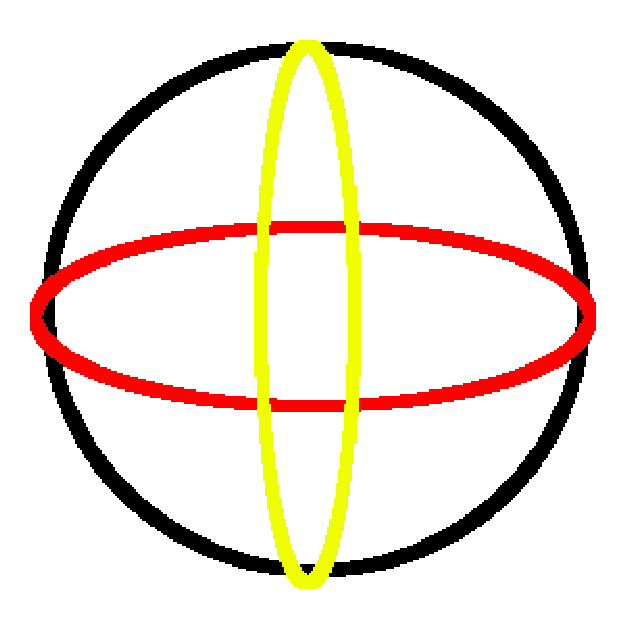
\includegraphics{3dof}
\caption {Three Degrees of Freedom}
\end{figure}
\begin{figure}[1dof]
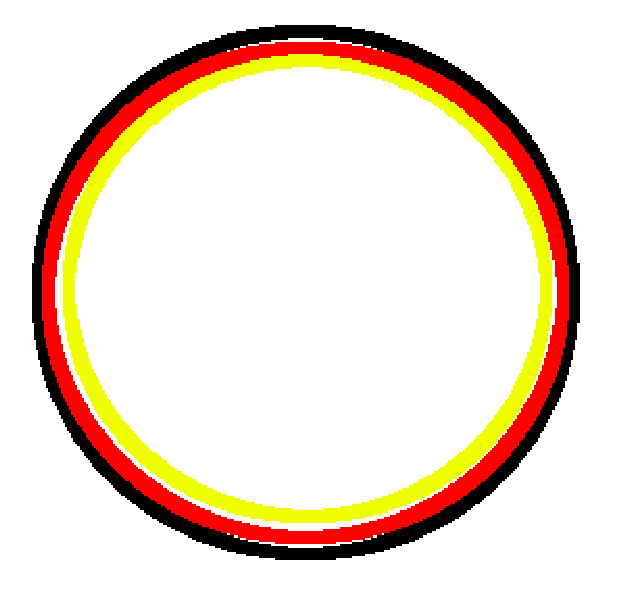
\includegraphics{1dof}
\caption {One Degree of Freedom}
\end{figure}

The three dimensional model
is useful in aerial and underwater environments and environments with
extreme slopes.  In most other cases, roll, pitch and the vertical
component of motion are considered systematic noise.

\section{Kinematic Model}

Consider motion from an initial pose $<x_{t_0} y_{t_0}\theta_{t_0}>$
with a velocity $v$. We want to know pose $<x_{t_{dt}} y_{t_{\delta t}}
\theta_{t_{\delta t}}>$ at time $\delta t$. Velocity is the first derivative of
position r with respect to time, $v = \frac{dr}{\delta t}$. We can pick out
the $x$ and $y$ components of motion with the coefficients $\cos
(\theta)$ and $\sin (\theta)$ respectively and determine the
displacement along each axis by integration. Adding that displacement
to the intitial position gives the new position. The the $x_{t_{\delta t}}$
position is thus $x_{t_0} + \int\limits_0^t v \sin (\theta) \mathrm{d}t$,
the $y_{t_{\delta t}}$ position is $y_{t_0} + \int_0^t \! v \cos (\theta) \,
\mathrm{d}t$. The heading remains constant. This is known as translation.

If the angular velocity $\omega$ is non-zero and the linear velocity is
zero, the position is constant, but the change in heading becomes
$\theta' = \int\limit_0^t \omega dt$. This is known as rotation.

Simultaneous translation and rotation complicates the model. Assume
that the robot travels with a constant velocity for a time interval
$dt$. \footnote{This is a realistic assumption for almost all
  scenarios where the interval is small enough.}  Rather than moving
along a line or on a point, it now moves along an arc $A$ with a
radius $r$. The length of the arc is $vdt$. The tangential (linear)
velocity is $v = r\omega$.  The radius is then $r = \frac{v}{\omega}$.
We also know the center of the circle is $<x_c y_c>$ where $x_c = x_t_0 -
r \sin (\theta)$ and $y_c = y_t_0 + r \cos (\theta)$.  We can calculate
the position of the robot along the edge of the circle by:

\begin{equation}
\label{motion_model}
\vec{x}_{t+1}=
\begin{pmatrix}
  x_c + r sin(theta + \omega \delta t) \\
  y_c - r cos(theta + \omega \delta t) \\
  \omega \delta t
\end{pmatrix}  +
\end{equation}

However, \ref{motion_model} does not generalize to the linear case. If
the angular velocity is 0, the radius is infinite and
\ref{motion_model} is undefined. In this case, we must use:

\begin{equation}
\label{motion_linear}
\vec{x}_{t+1} =
\begin{pmatrix}
 x + v \sin (\theta) \delta t\\
 y + v \cos (\theta) \delta t\\
 \omega
\end{pmatrix}
\end{equation}

\section{Drive models}
The most common drive systems for mobile robots are differential
drives and cars. They are well suited to indoor and outdoor
environments respectively.

The motion of a differential drive comes from the velocity of its two
wheels and their relative distance.  Consider a differential drive
robot traveling along an arc.  Rotation results from a difference in
speed between the right and left wheel and is proportional to the
distance between those wheels $l$.  Linear velocity is simply the
average of the two wheel velocities. \cite{Dudek}

\begin{equation}
\label{differential_drive_rotation}
\omega = \frac{v_r - v_l}{l}
\end{equation}

\begin{equation}
\label{differential_drive_velocity}
v = \frac{v_r + v_l}{2}
\end{equation}

%\begin{comment}
%TODO: Show transformation to particle
%TODO: Car model
%TODO: Show transformation to particle
%end{comment}

\section{Observation}
The observation model describes sensor behavoir. While odometry
information can be considered a sensor in a strict sense, this
sections deals with observations about landmarks in the environment.
There are many kinds of sensors including sonar, lidar and
cameras. The details of perception are usually abstracted into range
and bearing measurements from the robot to a landmark. In the case of
camera vision, considerable pre-processing might take place in order
to make the measurements useful for SLAM. A sensor also has some noise
characteristic, which is usually determined by experimentation before
hand via repeated measurements from a stationary position. The noise
is assumed to be normally distributed.


Features in the environment are often represeted as a point cloud of
landmarks. A two dimensional point cloud is a $2xN$ matrix for N
landmarks. Each row represents the $x$ and $y$ value of some point. It
is often useful to add a third column to represent a correspondence
variable.  At successive observations, the order of observation may
change. A correspondence variable helps keep track of a landmark at
each step explicitly.

An range and bearing sensor returns a measurement consisting of the
relative distance and angle from the x axis of the sensor. If the
sensor is not front and center on the robot, a transformation needs to
be applied to move the observation in to the frame of reference of the
robot. Once the observation is in a frame relative to the robot, it
can be converted to a cartesian coordinate and transformed into a
global frame if desired.

\begin{equation}\label{pol2cart}
\begin{pmatrix}
 x \\ y \\
\end{pmatrix} =
\begin{pmatrix}
 r cos \theta \\ r sin \theta \\
\end{pmatrix}
\end{equation}

The inverse observation model is:

\begin{equation}\label{cart2pol}
\begin{pmatrix}
 r \\ \theta \\
\end{pmatrix}
\begin{pmatrix}
 \sqrt{x^2 + y^2} \\ arctan(\frac{x}{y}) \\
\end{pmatrix}
\end{equation}

%\begin{comment}
%TODO: Show transformation to global frame.
%\end{comment}

If landmarks are easily distinguishable, such as through a barcode,
the correspondence variable is simply used to sort the observation
vector. If correspondence is not known a priori, a clustering
algorithm can determine whether the landmark was previously observed
and if so, which is the most likely candidate. This technique is known
as data association.

A commonly used clustering algorithms is Maximum Likelihood (ML)fi. ML
determines the correspondence variable by $c^\hat = \argmax{c_t} p(z_t
| c_{1:t}, m, z_{1:t-1}, u_{1:t})$. This is simply the correspondence
variable with the highest probability of being correct. One might use
the Mahalanobis distance to find which landmarks are within some
distance $\alpha$, then among those, choose the one with the smallest
distance. This is the most likely candidate.

ML can give potentially inaccurate results in highly cluttered
environments. JCBB is more complex but more consistent. 
%\begin{comment}
%TODO: More
%JCBB!
%\end{comment}

\section{Probablistic Models}

The motion and observation models provide a starting point for a
probablistic description of robot motion. Used by themselves, the
error from each measurement will grow unbounded. In order to generate
a stochastic map \cite{cheeseman1987stochastic}, we combine the output
of the motion model and observation model into a vector representing
the mean estimate of the environment state. The mean estimate has the
following form $\mu = <x_r y_r \theta_r z_{x1} z_{y1} z_{ci}
... z_{xn} z_{yn} z_{cn}>$.

Consider a pair of features, each some uncertain distance from the
robot. The sensors measure the distance as some value with an
emperically determined error. The robot then moves to another position
and again observes these two landmarks. This second observation
reinforces the relationship between the landmarks, reducing the
uncertainty of their relative distance. This reduction in uncertainty
comes because the measurement error is inherent in the robot, so all
the landmarks share the same error. As a network of relationships
between landmarks and robot poses grows, the map tends towards an
accurate relative representation \cite{durrant2006simultaneous}. This
increasing certainty in landmark position allows the robot to
accurately determine its own position given an observation of a
feature it has seen before.

Probablisticaly, movement is described by:

\begin{equation}\label{predict_step}
p(x_{t}|x_{t-1},u_{t})
\end{equation}

This gives the probability of the robot being at a particular pose
$x_{t}$ given its last pose at time $t-1$ and a control input,
$u$. \footnote{A possible source of confusion is the use of $x$ as the
  pose variable; $x$ is a vector describing the position and heading
  angle, $[x,y]$.  This is separate from the $x$ of the Cartesian
  coordinates of the robot and should be clear from context.}

The corresponding probablistic observation is described by:

\begin{equation}\label{obs_stepA}
p(z_{t}|x_{t})
\end{equation}

This model gives the probability that there is something at position
$z$, accurately observed given the current pose of the robot,
$x$, at some time $t$.  Usually the robot will want to also keep track
of landmarks it has seen, so it is common to add a map $m$.

\begin{equation}\label{obs_stepA}
p(z_{t}|x_{t}, m_t)
\end{equation}

These probabilistic models provide a foundation for a
predictor-updater algorithm known as the Recursive Bayesian
Estimation\cite{SomeCitationHere}.  Based on a prior state estimation, plus new information
from observation and a control signal, a new state estimate is formed.

\begin{algorithm}     
\caption{Recursive Bayesian Estimation}
\label{Bayes_Filter}   
\begin{algorithmic}         
    \Require Prior estimate $prior(x_{t-1})$ \State Control signal
    $u_t$ \State Observation $z_t$ \For{$i = 0:t$} \State
             {$prediction(x_t) := \int p(x_t | u_t, x_{t-1})
               prior(x_{t-1}) dx_{t-1} $} \Comment{Prediction Step}
             \State {$correction(x_t) := \eta p(z_t | x_t)
               prediction(x_t)$} \Comment{Correction Step} \EndFor

\State\Return $correction(x_t)$
\end{algorithmic}
\end{algorithm}

Intuitively, the Bayes Filter involves the robot moving to a position
and making an educated guess of its location. It then incorporates
observation data to improve that guess More rigorously, the filter
begins with an initial estimate of the state $x_0$, which is used as
the initial prior. The state is represented by a probability density
function. We assume the state estimate is Gaussian, so the density
function is represented by a state estimate and covariance matrix. The
filter also requires a control signal $u_t$ and observation $z_t$. The
first step of the for loop predicts the new state of the environment
based on the robot's motion. In a static environemnt, the only thing
that should change is the robot's pose. We can use that assumption to
estimate what the observations should be. That estimate is compared to
the actual observations to determine how much information each new
observation contains. This creates a better estimate of the state. The
algorithm repeats until the system stops.

Because the two steps in the for loop of the Bayes Filter do not
usually have a closed form, it's not very useful in practice
\cite{ThrunPR}. A number of algorithms approximate the Bayes filter.
The most commonly used is the Extended Kalman Filter or EKF. The EKF
is similar to the simpler Kalman Filter, with the addition of a
linearization step that makes it applicable to non-linear systems.

\section{EKF}  
In order to implement the EKF, we need to begin with data structures.
First, we assume that the noise in the motion and observation models
is Gaussian. While this is not necessarily true, it does allow for the
relative simplicity of the EKF and a tractable estimate is often
preferable to a more precise estimate. We will also assume discrete
time steps with a constant interval. The mean state estimate $x$ is a
column vector that combines the robot's pose at the current time $t$
$R_t = <x_r, y_r, \theta_r>^T$ and the position of all the observed
features $f_i \in F$, $f_i = <f_ix, f_iy>^T$. It's length is $N$,
where $N^2$ is the length of the pose and the combined length of the
features. The covariance $P$ describes the the confidence in each
landmark's position and is square with N elements.

The EKF is built on the Kalman Filter (KF) with an additional
linearization step to allow for estimation involving non-linear motion
and observation models. We will begin with a derivation of the Kalman
Filter and then the changes necessary to create an Extended Kalman
Filter.

Kalman Filters are an approximation of the Bayes Filter. A pair of
models are used; the process model and the observation model. These
correspond to the motion and measurement models for a mobile robot.
The generalized process model is:

\begin{equation}\label{kf_process_mean}
x_{t+1} = Fx_k + Gu_t + \epsilon
\end{equation}

\begin{equation}\label{kf_process_cov}
P_{t+1} = FP_tF^T + Q
\end{equation}

Here, the state at time $t+1$, $x_{t+1}$ is determined by the state
transition matrix $F$ applied to the prior state estimate $x_k$ plus
the control signal $u$ modified by some gain matrix $G$ along with
some Gaussian noise $\epsilon$ with a mean of 0 and covariance $Q$.
Just like the Bayes Filter, this step makes the best initial guess of
the state at the next instance. This is then corrected by using the
observation model. That model uses an observation $z$ at time $t+1$:

\begin{equation}\label{kf_observation}
z{t+1} = Hx_{t+1} + \gamma
\end{equation}

Here, $H$ is a matrix describing the observation process and 1y
is Gaussian noise with a mean of 0 and covariance $R$.

Prior to the update step, two new values are needed. The first is the
innovation covariance $S$ and the second is the Kalman gain $K$.
Innovation is a distribution indicating the difference between the
expected observation in \ref{kf_observation} and the actual
measurement. It is how much information a new observation provides for
the filter, modified by a gain which is proportional to the current
confidence in the estimate of a feature.  The formulas for $S$ and $K$
respectively are:

\begin{equation}\label{kf_innovation}
S = HP_{t+1}H^T + R
\end{equation}

and

\begin{equation}\label{kf_gain}
K = P_{t+1}H^TS^{-1}
\end{equation}

The update step uses this observation value to make a new state
estimate:

\begin{equation}\label{kf_update}
\hat{x}_{t+1} = x_{t+1} + K(z_{t+1} - Hx{t+1}
\end{equation}

\begin{equation}\label{kf_update_cov}
\hat{P}_{t+1} = P_{t+1} - KSK^T
\end{equation}


The trouble with the Kalman Filter is that it is only applicable to
linear Gaussian processes, and the motion and observation models for a
mobile robot are certainly not linear, due to the presence of
transcendental functions. A modification is necessary to use the
Kalman Filter for SLAM. Rather than a state transition matrix and an
observation matrix, the Extended Kalman Filter uses two differentiable
non-linear functions.

\begin{equation}\label{ekf_f}
x_{t+1} = f(u_t, x_t) + \epsilon
\end{equation}

\begin{equation}\label{ekf_h}
z_{t+1} = h(x_{t+1}) + \gamma
\end{equation}

In the prediction step, the initial state estimate is simply the
result of $f$. But in order to compute the covariance $P_{t+1}$,
$f(u,x)$ needs to be linearized. This is done by computing the
Jacobian matrix $\nabla f$, which is the total derivative of $f$
evaluated at $x_t, u_t$. The resulting function is a plane tangential
to $f$ that is a reasonable approximation. The estimate for $P_{t+1}$
is then calculated by:

\begin{equation}\label{ekf_cov}
P_{t+1} = \nabla fP_t \nabla f^T + R
\end{equation}
The observation model is linearized in the same way, with the
resulting Jacobian matrix $\nabla h$.

The Innovation matrix and Kalman gain are calculated by:

\begin{equation}\label{ekf_S}
S = \nabla h P_{t+1} \nabla h^T + R
\end{equation}

\begin{equation}\label{ekf_K}
K = P_{t+1} \nabla h^TS^{-1}
\end{equation}

The final state estimate and covariance are the same as the Kalman
Filter.

The complete EKF algorithm is as follows:

\begin{algorithm}     
\caption{Extended Kalman Filter}
\label{EKF}   
\begin{algorithmic}         
    \Require Prior Estimate $x_{t-1}$ 
    \Require Prior Covariance $P_{t-1}$
    \Require Control signal $u_t$ 
    \Require Observation $z_t$
    \Require Motion Noise $Q$
    \Require Observation Noise $R$

    \begin{comment} Prediction    \end{comment}
    \State $\hat{x} = f(u, x_{t-1})$
    \State $F = f'(u,x_{t-1})$
    \begin{comment} Update \end{comment}
    \State $y = z - h(\hat{x})$
    \State $\hat{P} = F * P_{t-1} * F^T + Q$
    \State $H = h'(z_t)$
    \State $S = H * \hat{P} * H' + R$
    \State $K = P\hat * H' * S^{-1} +Q$  
    \State $x = \hat{x} + K * y$
    \State $P = P\hat - K * S * K'$

\State\Return $(x, P)$
\end{algorithmic}
\end{algorithm}


Some additional work is necessary to do SLAM with the EKF. To begin,
odometry and sensor data is necessary.\footnote{ It is convenient to
  have a simulator to create this data. The source code for such a
  simulator is provided in the appendix.} If multiple observations are
made at each step, the update step must occur for each observation.
If data association is unkown, this must be done at some point prior
to the EKF prediction and correspondence variables must be assigned.

The Extended Kalman Filter, while the most common method for state
estimation, does have some serious flaws.  While it is known to
converge on an estimate, \cite{HuangEKFAnalysis} it turns out to be
inconsistent over a large number of time steps.  The linear Kalman
Filter converges and is consistent, because no approximations are
necessary.  In order to fit the non-linear motion and observation
functions into the framework of the KF, the linearization step is
necessary.  Because the Jacobian matrix used for the linearization
step is calculated using the state estimate and not the true state,
it might be very inaccurate.  Because the EKF does not account for
this, it may become overconfident in it's estimate and the true
position of a landmark might lie outside the ellipse described by the
covariance matrix.

While the EKF works well for small indoor environments, it's
inconsistentcy makes it wholly unsuitable for large scale
environments.  Additionally, it suffers in large environments because
every landmark is considered in the covariance update, even when they
are not in the set of local observations.  Advancements in SLAM
algorithms focus on local updates and keeping the covariance matrix
sparse, in order to take advantage of spare linear algebra methods.


\chapter{State of the Art}

A good SLAM algorithm must have several properties. It need to be fast
enough for real time processing. It needs to perform well in very
large environments\cite{iSAM}. Finally, it needs to support online
data association. There are numerous algorithms that, while
technically interesting, do not meet one or more of these
criteria. One method has emerged as the de-facto SLAM
backend\footnote{In real-time robotics, the SLAM system consists of a
  front end which handles the measurements and converts them to form
  suitable for processing. The back end is the algorithm responsible
  for actually doing SLAM.}- Incremental Smoothing and Mapping
\cite{iSAM} (iSAM).

iSAM, based on the earlier Square Root Smoothing and Mapping, breaks
from other methods by using smoothing rather than filtering to
determine the correct state estimate. It also tracks the robot
trajectory, which ironicly improves accuracy without sacrificng
computational simpicity. This tends to be faster than the EKF around
600 landmarks \cite{Dellaert06ijrr}. Because it uses the entire data
set, it provides an optimal estimate given the measurements
available. Thus it does not suffer from the linearization errors and
inconsistency of the EKF.

iSAM is also often used as a map optimization tool for graph based
SLAM applications \cite{Sunderhauf}. A mobile robot that is operating
in an environment can add nodes and edges to a graph, just as in
GraphSLAM.  Once the map is needed for planning, iSAM can be run on
the graph, even if the graph is extremely large, and return a result
in a matter of seconds. While this is still not quite fast enough to
make some time critical decisions, it is a great leap forward for SLAM
algorithms.

The first step in understanding iSAM is reformulating the SLAM problem
as a least squares problem that finds the maximum a posteriori
estimate of the trajectory and landmarks. It is important to note that
this formulation is non-linear. We find the estimated trajectory $T^*$
and landmarks $L*$ by $\argmin{T,L} \{\sum_{i=1}^M (f_i(x_{i-1}, u_i)
- x_i)^T \Lambda (f_i(x_{i-1}, u_i) - x_i) + \sum_{k=1}^K (h_k(x_{ik},
l_{ij}) - z_k)^T \Gamma (h_k(x_{ik}, l_{ij}) - z_k)\}$ Because this is
a non-linear least squares formula, finding the minimum first involves
an interative optimization algorithm such as Gauss-Newton to estimate
the the process and measurement models as linear functions.

%\begin{comment}
%TODO: Move from Least Squares section to here
%\end{comment}

In order to run in real time, iSAM solves the initial problem for the
initial pose observations by QR Factorization and applying a rotation
matrix to all of the submatrices such that the resulting information
matrix is in upper triangular form. As new measurements are added,
another rotation is applied to resume the upper triangular form. At
any time, the result of the QR factorization can be used to recover
the estimated trajectory and map.

Several small improvements have been made to iSAM to improve its run
time, but any drastic improvements are more likely to come from
techniques that approximate the information matrix.

Iterated Sparse Local Submap Joining (I-SLSJF) is yet another approach
that tries to reduce the complexity of SLAM. In this case, the
reduction comes from dividing the problem into a series of overlapping
submaps \cite{huang2008iterated}. Where graph based SLAM first
estimates a graph of poses, submap joining works more like traditional
SLAM in that it focuses on the estimation of feature locations. As a
side effect of the submap joining process, a coarse estimate of the
robot trajectory is produced. But because the entire trajectory is not
maintained, the number of dimensions in the problem is greatly reduced
when compared to other batch SLAM solutions.

Submaps are usually produced with an EKF or other simple estimation
technique and consist of a single step with a start and end pose in a
local frame of reference. The end pose of a map is always the start
pose of the next map in order to facilitate the fusing process. The
initial version of the algorithm uses an information filter to match
observations shared between maps. This filtering can still suffer from
some linearization errors, so if an inconsistency is detected at any
step, it can apply smoothing to the global map to recover from this
inconsistency.

Another area of very active research is cooperative multi-robot
mapping \cite(wang2007multi) \cite(multiSEIF), \cite(4399142),
\cite(4543634), \cite(5509154). Outside of SLAM research, robot groups
are popular because of improved redundancy and the obvious benefits of
being able to execute a task in a distributed manner. Often
multi-robot systems consist of lower cost components because the group
as a whole has a higher fault tolerance than any individual member. If
an individual fails, the impact on the completion of the overall goal
is mitigated. This can be useful in situations where the individual
chance of failure is relatively high, or the cost of failure is high.

There are two challenges associated with multi-robot SLAM:
distinguishing robots from landmarks and the determination of a shared
frame of reference. Mistaking a robot for a landmark and adding it to
the map can lead to an extremely inconsistent landmark. If a robot in
the team is observed and classified as a landmark in one location and
then observed again at another location, the observer may conclude
that a loop has been closed, when this has in fact not occurred. The
simplest way to cope with this is for the team to have a priori
knowledge of the other members and devise some way to uniquely
distinguish them from the environment, such as a barcode or unique
pattern of infrared flashes. The other alternative is to make the SLAM
implementation robust in a dynamic environment, but this comes with
unique data association challenges.

Determination of a shared reference frame can be done by sharing maps
when a mutual pose observation occurs between two or more robots. Once
a robot determines that it has observed another robot, it can
communicate with the other team member and share its map and current
pose estimate. In the map thus shared, there will be an estimate of
the position of the team member. This point can then be used like the
shared start end end poses with I-SLSJF SLAM. Once the location of the
two robots is determined, it becomes possible to calculate the correct
rotation and translation vectors to align the shared map with the
robot's local map.

%\begin{comment}
%C-SAM
%Multiple Relative Pose Graphs
%\end{comment}

\section{Map Joining}
The map joining approach to SLAM relies on the creation of submaps:
local maps focused only on a subset of a trajectory and the
immediately related observations. The creation of local maps is
usually accomplished by either Extended Kalman or Information Filters.
Markov Chain Monte Carlo methods have also been suggested . While
these methods prove to be inconsistent, this inconsistency is only
significant in large sets of observations. By limiting their scope,
linearization errors, inconsistency and complexity can be held in
check. The earliest paper I have found on map joining is
\cite{tardos2002}. This describes the fundamental operations of map
joining: transformation from a common observation into a global
coordinate frame and feature association. More recent formulations
\cite{c-sam} have eliminated the need for explicit transformation
through the use of a graph theoretic formulation of SLAM. In this
case, the more general term ‘map alignment’ is used over
transformation. No matter how the maps are aligned, the second step is
data association. Because of possible noise in the observation of a
common landmark, alignment may not place all landmarks at the same
point. This requires a classification algorithm to be run over the
map, such as k-Nearest Neighbor or Joint Compatibility Branch and
Bound \cite{tardos2002}. Other classifiers can be used, but are not
common in the literature. Classification can be eliminated if
noiseless identification of features is possible, such as when using
cameras and unambiguous barcodes. If there are common landmarks
between the two submaps, after classification, a new state estimate is
required to make sense of the matched but non-coincident features.
This is accomplished by calculating a least squares estimate of the
new global map, to create a best fit ‘curve’ describing all the
observations.

\section{ Spherical Matrices, One Step SLAM and Map Joining}
A key observation to the reduction of dimensionality in single step
SLAM is the use of spherical covariance matrices. An spherical matrix
is defined as any matrix that is commutative with a rotation matrix. A
rotation matrix R(theta) is [cos t -sin t; sin t cos t]. For all theta
and any spherical matrix A, AR = RA.

It is important that the covariance matrices are also positive
definite. A matrix is positive definite if for all positive, non-zero
column vectors $v, v^T Mv > 0$. This is to allow for methods analogous
to finding the square-root of a matrix, such as Cholesky or QR
factorization to be used in the solution of the least squares
estimate. In the Automatica preprint, Dr. Huang claims that this
objective function, when applied to single step SLAM, is equivalent to
a one dimensional optimization problem. Through repeated application
of single step SLAM for each timestep, an approximate solution to the
previous objective function can be easily found. It is approximate
because a spherical covariance matrix is used, rather than the actual
covariance associated with observation uncertainty. In On The Num of
Local Minima, Dr. Huang shows that single step SLAM and map joining
SLAM share the same property of having only 1 or 2 minima, one of
which is global, when covariances are approximated by spherical
matrices. This provides the benefits of the reduction in linearization
error due to map joining, along with the low dimensionality of single
step SLAM. Additionally, if multi-robot map joining belongs to this
class of problems, map sharing can possibly become quite efficient. In
a remark from \cite{onthenumber}, Huang notes that the covariance
matrices must only be spherical, but not identical. That is, the
covariance can differ for each odometry measurement and observation.
This lends some home to the possibility that multi-robot map joining
is in this class of problems.

\section{SLAM and Machine Learning}

There are two sub-problems within SLAM that call for the
application of machine learning techniques, landmark
association and least squares optimization. These are two
separate types of problems, the former being unsupervised
classification, the latter is convex optimization.

Landmark association, also known as data association, is a
classification problem that uses a pair of feature maps or a map and
set of observations and tries to match known landmarks with new
observations. In most cases, this is an unsupervised learning problem
because the set of features can vary so greatly from map to map, it is
not possible to provide examples for a supervised approach. This is
necessary for any environment where there can be ambiguity in
landmarks. While it might be possible in a lab to put barcodes on
landmarks that can be recognized with a camera, in scenarios where a
camera might not be available or barcoding landmarks unfeasible,
landmark association is required. The least squares portion of SLAM is
non-linear and of a very high dimension. Because of this, single step
techniques such as linear regression are not applicable. Other
algorithms such as Levenberg-Marquardt, Gauss-Newton and Stochastic
Gradient Descent must be used instead. These three methods are the
most popular among SLAM researchers.

The Gauss-Newton method is used effectively in iSAM \cite{isam}. It is
a variation on Newton’s method for finding the minima of a function
taught in elementary calculus courses but is modified to solve least
squares problems. It begins with an initial guess $x_0$ of a possible
solution. For an objective function $f(x)$ and a residual function
$r(x)$, the jacobian at $r(x_0)$ is calculated. The jacobian is a
linearization estimate of $r(x)$ and is used for the next guess. This
process is repeated until it converges on a solution. It is possible
in certain situations to overshoot the optimum and fail to converge.
This algorithm can also fail to find a global optimum and instead
converge on a local optimum.

Gradient descent is an optimization algorithm similar to hill
climbing, but rather than selecting a single element to improve, it
follows the slope (or gradient) of the function towards a solution.
Like Gauss-Newton, gradient descent can get stuck in local optima. A
modification known as stochastic gradient descent can overcome this
limitation.


\chapter{Methods}
\section{Robotic Data}
The experiment uses the UTIAS multi-robot data set. The data consists
of odometry as linear and angular velocities, and feature observations
as range and bearing relative to the center of the robot along its
line of motion. This was produced by six iRobot Creates, each with a
monocular camera mounted on the center of the robot along the local
x-axis. Each robot was marked by a vertical barcode to allow for easy
identification of other agents.

The landmarks were posts with barcodes similar to those on the robot
chassis. The number of landmarks varried between N and M, and were
arranged in different configurations for each system. A total of nine
sets are provided.

Groundtruth for landmarks was provided, along with groundtruth for the
robots at each measured time. Groundtruth was gathered by an accurate
object tracking system with an approximate accuracy of 1 mm.

The data set provided a script for sampling from the data sets and
interpolating to provide a consistent interval. Early work with this
data showed that very small intervals too much data for the available
disk space and processing power.

The data as available was preprocessed to allow for easy intgration
with backend slam algorithms. Range and bearing information was
extracted from the images. images were provided but not used. Odometry
information was converted from differential drive form to the particle
model.

Prior to experimentation, some additional work was necessary. In some
data sets there were erroneous measurements that needed to be removed.
the data was sampled and interpolated into one second intervals.


\section{Simulator}
In order to test the map joining algorithm with a large collection of
features, a point mass robot simulator is used. The simulator creates
a set of uniformly random landmarks and uniformly random waypoints
within a particular radius. The size of the sets and radius are
configurable. The sensor is a range and bearing sensor with a range of
10 meters and covers an arc of $\pi/4$ radians.

The simulator starts with an initial observation before any motion.
The robot rotates towards the first waypoint and then heads towards it
with a maximum velocity of one meter per second. Once the robot
reaches the waypoint, the process repeats until the robot reaches the
final landmark, when the simulation ends. Observations occur every
second, immediately after the motion step. The resulting odometry and
observation data is formatted identically to that used in the UTIAS
data set. The simulator was run thirty times each for landmark counts
of 10 and 100.

\section{Experiments}
The first experiment was to create single robot maps using just the
EKF algorithm from THRUN. The algorithm assumes known and correct,
noise free data association. while not true in most realistic
operating environments, the simplifying assumption allows map quality
to be assessed without confounding factors. The results from this
experiment are the baseline for those that follow. Accuracy of the
estimation is calculated for both the map and the trajectory using the
root mean squared error (RMSE) technique to measure how close the
estimate was to the available groundtruth. The average RMSE of all
runs in both the UTIAS data set and all the runs in the simulated data
set is calculated and used as the benchmark.

The next experiment was single robot map joining. The purpose of this
experiment is to record the accuracy improvements of the map joining
approach over the EKF alone. Using the EKF, a submap was saved at each
time step. The submap is just a snapshot of the current state
estimate. Prior to prediction phase, the state estimate is cleared of
all landmarks to preserve the independence of each submap. Only the
mean estimate of features and the ending pose are saved. The
covariance is discarded because it will be estimated by an identity
matrix during the map joining phase. This results in a space savings
of 144 Kb for each submap with a state vector of 48 elements, assuming
64 bit doubles. Map joining was done offline after all submaps were
collected.

Offline map joining was accomplished by the algorithm described in
cite{HUANG}. The algorithm keeps track of the global map state and a
single robot's trajectory. Map joining is accomplished by a by finding
the state $X_{join}$ that satisfies the least squares problem

\begin{equation}
\underset{X_{join}}{\operatorname{argmin}} \sum \limits_{j=1}^k
(\hat{X} - H(X_{join})^T) P^{-1} (\hat{X} - H(X_{join}))
\end{equation}

Optimization is done with the Matlab optimization toolbox {Cite},
using the Quasi Gauss Newton algorithm {Cite}. This algorithm was
selected because it is the simplest optimization method for a function
with a single minimum. While this may fail in the case of two local
minima, that will only occur if data association is very poor. Because
the maps all have completely accurate data association, that condition
will not occur. Accuracy for the trajectory and map are determined by
comparing the resulting estimates to groundtruth and computing the
RMSE, just as with the EKF.

The final experiment was multi robot map joining. It followed the
lines of single robot map joining, except when another robot was
observed. At that time step, the local maps for each robot were
exchanged. Singlular value decomposition was used to determine the
ideal rotation matrix and translation vector. After applying that
transformation, the two maps are joined using the same function as
single robot map joining, except trajectory is ignored. Optimization
is also done with the Quasi Gauss Newton algorithm. Additional,
optimization is verified using a genetic algorithm as a global
optimization technique. If the shared map joining least squares
problem has only one local minima, the resulting estimate will be
similar.

\chapter{Results}

\begin{figure}
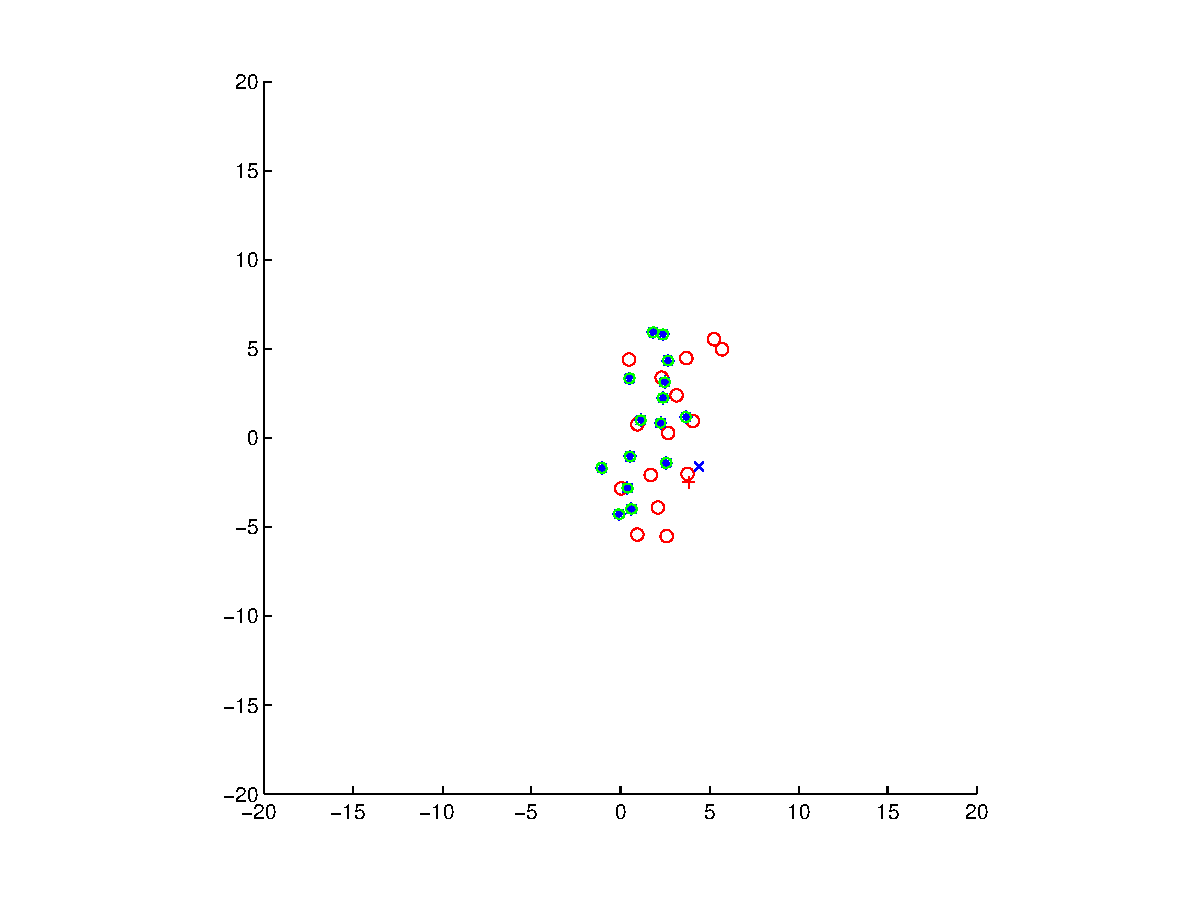
\includegraphics{mapsample}
\caption{Sample EKF Map}
\end{figure}
The first experiment, single robot EKF, had nine data sets with five
robots each, for a total of forty-five maps that were created. The
aggregate Root Mean Squared Error between the map and groundtruth is
0.4004 m with a standard deviation of 0.0806 m. The details for each
run are shown in table 4.1. The aggregate RMSE of the trajectory
estimate and groundtruth is 0.0462 m with a standard deviation of
0.0074 m.

The second experiment, single robot map joining has an aggregate RMSE
of 0.0347 meters and a standard deviation of 0.0164 meters. As with
the EKF experiment, this was done with nine data sets each with five
robots, for a total of forty-five maps. The mean RMSE of the trajecory
compared to groundtruth is 7.7e-5 meters with a standard deviation of
4.9e-5 meters. A paired T test of the hypothesis that the mean RMSE of
the first experiment's map is equal to the RMSE of the second
experiment's map with 95\% confidence gives a p-value of 3.04e-4.

The third experiment, multi-robot map joining has an aggregate mean
RMSE of 0.0467 meters and aggregate standard deviation of 0.0240
meters. Trajectory was not considered in this experiment. A pairted T
test of the hypothesis that the mean RMSE of the single robot map
joining experiment is equal to the mean RMSE of the multi-robot map
joining experiment at a 95\% confidence interval gives a p-value of
0.1018.

\begin{center}
\begin{table}[h]
  \caption{Root Mean Square Error of Single Robot EKF Maps in Meters}
  \begin{tabular}{| l | c | c | c | c | c || r ||r |}
    \hline Set & Robot 1 & Robot 2 & Robot 3 & Robot 4 & Robot 5 &
    Average RMSE & Std Dev \\ \hline \hline 1 & 0.3304 & 0.4240 &
    0.2255 & 0.3733 & 0.2437 & 0.3194 & 0.0844\\ \hline 2 & 0.3990 &
    0.1655 & 0.6744 & 0.3071 & 0.5666 & 0.4225 & 0.2026\\ \hline 3 &
    0.0599 & 0.4383 & 0.7593 & 0.5151 & 0.4371 & 0.4419 &
    0.2510\\ \hline 4 & 0.2483 & 0.3933 & 0.5499 & 0.3501 & 0.2237 &
    0.3531 & 0.1305\\ \hline 5 & 0.1555 & 0.3135 & 0.3689 & 0.5330 &
    0.3344 & 0.3411 & 0.1350\\ \hline 6 & 0.6738 & 0.5618 & 0.5167 &
    0.5235 & 0.5974 & 0.5746 & 0.0642\\ \hline 7 & 0.4676 & 0.1768 &
    0.2946 & 0.5613 & 0.3348 & 0.3670 & 0.1503\\ \hline 8 & 0.2980 &
    0.2922 & 0.1912 & 0.7909 & 0.1180 & 0.3381 & 0.2640\\ \hline 9 &
    0.1874 & 0.7517 & 0.5520 & 0.5976 & 0.1405 & 0.4458 &
    0.2683\\ \hline \hline RMSE & 0.3133 & 0.3908 & 0.4592 & 0.5058 &
    0.3329 & - & -\\ \hline Std Dev & 0.1840 & 0.1854 & 0.1994 &
    0.1480 & 0.1727 & - & -\\ \hline \hline
  \end{tabular}
  \end{table}
\end{center}

\begin{center}
\begin{table}[h]
  \caption{Root Mean Square Error of Single Robot EKF Trajectory}
  \begin{tabular}{| l | c | c | c | c | c || r ||r |}
    \hline Set & Robot 1 & Robot 2 & Robot 3 & Robot 4 & Robot 5 &
    Average RMSE & Std Dev \\ \hline \hline 1 & 0.0393 & 0.0353 &
    0.0399 & 0.0450 & 0.0419 & 0.0403 & 0.0036\\ \hline 2 & 0.0526 &
    0.0352 & 0.0467 & 0.0362 & 0.0455 & 0.0433 & 0.0074\\ \hline 3 &
    0.0391 & 0.0381 & 0.0620 & 0.0602 & 0.0347 & 0.0468 &
    0.0132\\ \hline 4 & 0.0437 & 0.0412 & 0.0412 & 0.0516 & 0.0479 &
    0.0451 & 0.0045\\ \hline 5 & 0.0281 & 0.0300 & 0.0327 & 0.0318 &
    0.0368 & 0.0319 & 0.0033\\ \hline 6 & 0.0563 & 0.0557 & 0.0634 &
    0.0609 & 0.0474 & 0.0567 & 0.0061\\ \hline 7 & 0.0563 & 0.0452 &
    0.0418 & 0.0755 & 0.0466 & 0.0531 & 0.0136\\ \hline 8 & 0.0391 &
    0.0381 & 0.0620 & 0.0602 & 0.0347 & 0.0468 & 0.0132\\ \hline 9 &
    0.0415 & 0.0672 & 0.0471 & 0.0595 & 0.0420 & 0.0514 &
    0.0114\\ \hline \hline RMSE & 0.0440 & 0.0428 & 0.0485 & 0.0534 &
    0.0422 & - & -\\ \hline Std Dev & 0.0094 & 0.0117 & 0.0013 &
    0.0137 & 0.0050 & - & -\\ \hline \hline
  \end{tabular}
  \end{table}
\end{center}

\begin{center}
\begin{table}[h]
  \caption{Root Mean Square Error of Single Robot Joined Maps in
    Meters}
  \begin{tabular}{| l | c | c | c | c | c || r ||r |}
    \hline Set & Robot 1 & Robot 2 & Robot 3 & Robot 4 & Robot 5 &
    Average RMSE & Std Dev \\ \hline \hline 1 & 0.0501 & 0.0055 &
    0.0110 & 0.0164 & 0.0146 & 0.0195 & 0.0176\\ \hline 2 & 0.0268 &
    0.0031 & 0.1410 & 0.0312 & 0.1102 & 0.0625 & 0.0596\\ \hline 3 &
    0.0044 & 0.0296 & 0.0647 & 0.1097 & 0.0123 & 0.0441 &
    0.0434\\ \hline 4 & 0.0345 & 0.0212 & 0.0046 & 0.0008 & 0.0302 &
    0.0183 & 0.0150\\ \hline 5 & 0.0308 & 0.0497 & 0.0680 & 0.0140 &
    0.0609 & 0.0447 & 0.0222\\ \hline 6 & 0.0337 & 0.0220 & 0.0054 &
    0.0000 & 0.0310 & 0.0184 & 0.0151\\ \hline 7 & 0.0337 & 0.0220 &
    0.0054 & 0.0000 & 0.0310 & 0.0184 & 0.0151\\ \hline 8 & 0.0419 &
    0.0484 & 0.0004 & 0.1284 & 0.0114 & 0.0461 & 0.0502\\ \hline 9 &
    0.0246 & 0.0723 & 0.0910 & 0.0049 & 0.0088 & 0.0403 &
    0.0390\\ \hline \hline RMSE & 0.0312 & 0.0304 & 0.0435 & 0.0339 &
    0.0345 & 0.0347 & 0.0308\\ \hline Std Dev & 0.0119 & 0.0212 &
    0.0473 & 0.0467 & 0.0308 & 0.0155 & 0.0164\\ \hline \hline
  \end{tabular}
  \end{table}
\end{center}

\begin{center}
\begin{table}[h]
  \caption{Root Mean Square Error of Single Robot Smoothed Trajectory
    in Meters}
  \begin{tabular}{| l | c | c | c | c | c || r ||r |}
    \hline Set & Robot 1 & Robot 2 & Robot 3 & Robot 4 & Robot 5 &
    Average RMSE & Std Dev \\ \hline \hline 1 & 1.3e-4 & 2.8e-5 &
    3.5e-5 & 1.4e-4 & 6.1e-6 & 6.7e-5 & 6.2e-5\\ \hline 2 & 1.1e-4 &
    5.1e-5 & 7.1e-6 & 1.2e-4 & 3.7e-5 & 6.5e-5 & 4.8e-5\\ \hline 3 &
    1.4e-4 & 6.2e-6 & 2.0e-5 & 2.1e-4 & 2.4e-5 & 8.1e-5 &
    9.1e-5\\ \hline 4 & 1.5e-4 & 1.5e-5 & 7.0e-5 & 1.6e-4 & 2.2e-5 &
    8.4e-5 & 7.0e-5\\ \hline 5 & 5.8e-6 & 9.1e-6 & 6.2e-6 & 2.3e-5 &
    2.6e-5 & 2.4e-5 & 2.1e-5\\ \hline 6 & 3.6e-5 & 7.5e-5 & 1.8e-4 &
    3.0e-5 & 1.8e-4 & 2.2e-4 & 1.1e-4\\ \hline 7 & 2.0e-5 & 9.4e-5 &
    1.7e-5 & 1.5e-4 & 6.0e-6 & 9.2e-5 & 8.2e-5\\ \hline 8 & 6.8e-7 &
    1.5e-5 & 2.2e-5 & 2.8e-6 & 2.3e-5 & 1.4e-5 & 9.0e-6\\ \hline 9 &
    1.6e-6 & 1.4e-5 & 1.0e-4 & 1.3e-5 & 7.6e-5 & 4.4e-5 &
    4.2e-5\\ \hline \hline RMSE & 6.6e-5 & 3.4e-5 & 5.1e-5 & 9.4e-5 &
    4.5e-5 & 7.7e-5 & 6.0e-5\\ \hline Std Dev & 4.7e-5 & 3.7e-5 &
    6.8e-5 & 5.2e-5 & 8.3e-6 & 7.0e-5 & 4.9e-5\\ \hline \hline
  \end{tabular}
  \end{table}
\end{center}

\begin{center}
\begin{table}[h]
  \caption{Root Mean Square Error of Multi Robot Map Joining in
    Meters}
  \begin{tabular}{| c | c | c | c | c | }
    \hline Set 1 & Set 2 & Set 3 & Set 4 & Set 5\\ \hline 0.0480 &
    0.0617 & 0.0254 & 0.0392 & 0.0726\\ \hline Set 6 & Set 7 & Set 8 &
    Set 9 & -\\ \hline 0.0103 & 0.0335 & 0.0423 & 0.0877 & - \\ \hline
    Mean & StdDev & & & \\ \hline 0.0467 & 0.0240 & & & \\ \hline
  \end{tabular}
  \end{table}
\end{center}



\chapter{Discussions}

The performance of the EKF for single robot mapping is poor relative
to the map joining approach. For comparison, the diameter of an iRobot
Create is approximately 0.35 meters and the EKF error was 0.40 meters.
Upon visual inspection, it appears that the maps may be similar but
require a two-dimenional transformation to accurately represent
groundtruth. Of course, this is not possible to determine that
transformation if groundtruth is not available.

The two possible explanations for this are an inaccurate initial pose
and linearization errors. In the case of the experiment using the
UTIAS data set, an accurate initial pose for each robot was available.
The discrepancy must be due to linearization errors then. This,
combined with the overconfidence of the EKF means the robot cannot
recover from this error and will continue to converge on an inaccurate
map.

The accuracy is acceptable, considering the very slow monocular camera
and imprecise odometry on the Create platform, for tasks where a
Create might be used. But it turns out that drastic impreovements are
realized when using the map joining approach. For these experiments,
the resulting accuracy improves by an order of magnitude. This result
is within the radius of the robot's chassis, which is a nice first
pass heuristic for the expected accuracy. The Quasi-Newton algorithm
has a complexity of $O(n^2)$ \cite{matlab} for n dimensions. This is
less than the $O(n^3)$ of the EKF, so it does not add any additional
complexity to the process. Additionally, the optimization step only
took 2.98 iterations on average and never more than 3 iterations.

Multi-robot map joining is not siginifcantly different from single
robot map joining. The lack of accuracy improvement is likely to due
to the map joining being a smoothing approach and thus already an
ideal estimator \cite{estimators}. While there is no improvement in
mapping accuracy, there is also no degredation when map data is shared
in a homogenous swarm. Trajectory is not considered when sharing maps
because tracking is not considered. Without modification, this
algorithm cannot improve on trajectory estimation because it relies on
landmarks being stationary over time.


\chapter{Conclusions}

Multi Robot map joining using least squares optimization works very
well in a homogenous swarm of robots. While some additional processing
is required over the traditional EKF SLAM approaches, it is a small
constant factor and does not add any complexity. That small factor
gives strong gains in maping accuracy. Compared to the time required
for the robot to make observations, the method shown here is fast
enough to be used in real time, even in an interpreted language such
as Matlab.
	
Another feature of this approach is the uniform method used for local
smoothing and map sharing. This method's dual use means the robot's
navigation system has, metaphorically, less moving parts to fail. This
is unique in the literature involving map joining SLAM \cite{slam}
Other map joining schemes use a separate algorithm for creating
individual maps and joining shared maps.

While this work focuses on two dimensional SLAM, it is applicable to
three dimensional environments as well.  It is believed
\cite{HuangICRA12} that map joining in $n$ dimensions has at most $n$
local minima.  However, because the other minima tend to be present
when data association is very poor, it is possible that the closed
form map joining algorithm is still applicable.
	
Finally, multi robot map joining is an iterative process that can be
picked up any time as resources are available. It can also be paused
and picked up again at any time, without adversely affecting the
results. The tradeoff is the space required for submap storage. While
non-submap techniques only require a single point for each map
feature, submapping requires an point to be stored for each
observation. However, even the Mars rover, Curiosity has 2GB flash
memory \cite{curiosity}, which is sufficient for the storage of
several large submaps prior to joining. The need for space is tempered
by the estimate of the covariance matrix. Because of this the submaps
need only store the estimate and not the covariance.
	

\chapter{Future Work}

Numerous tasks exist for future work implied by this thesis. The most
obvious is to extend this system to handle unknown data association.
While data association is a well studied subject, it adds considerable
complexity to the system. Three dimensional mapping is also important
for the usefulness of this system. Work is in progress showing that
map joining in three dimensions has at most two local minima
\cite{huang_icra12_talk}. This would require an efficient stochastic
optimization method to replace the Gauss-Newton method currently used.

Trajectory tracking is another important area. Having a multi robot
system provides an opportunity to add additional trajectory data, but
this also would add a great deal of complexity to the system. It is
not clear that this can be done within the current framework and may
require additional algorithms.

It is unknown whether multi-robot map joining requires homogenous
robots. Work on sensor fusion and learning the accuracy of various
robots on a heterogenous swarm could help answer this question.

Finally, an actual on-line system needs to be developed. The current
system works with the data after it has been collected and does not
work with the data as it arrives in real time streams. While I believe
this is an accurate model of the problem, it is not currently usable
on robots in real time.

\chapter{Appendix I: Simulator Source}
The following is MATLAB source code for a robot simulator.  The map is
considered a circle with some particlar radius, defined in the
``Configuration'' section.  A number of landmarks are randomly
generated. With the same algorithm, a number of waypoints for the
robot to travel to are also generated.  Sensor parameters including
range, arc and noise are also defined. 

 A parameter named ``close'' is
the maximum distance the robot can be away from a waypoint before it
moves to the next one.  This is a device to overcome floating point
rounding errors.

Some graphics code is included to show the landmarks, the estimate and
the robot's true and estimated positions during the run.  If this is
done to collect data, the removal of this section is recommended
because of speed considerations.

\singlespacing
\begin{verbatim}
SIMULATOR.M:
% Configuration
landmarks = 10;
waypoints = 100;
map_radius = 30;
dt = 1;
close = 1;

motion_noise = .001;
observation_noise = .01;

sensor_arc = pi/4; sensor_range = 10;

% Initialize
start_pose = [0;0;0];
start_time = 0;
map_true = create_points(map_radius, landmarks);
waypoint_list = create_points(map_radius, waypoints);

% Graphics
mapFig = figure(1);
axis([-map_radius map_radius -map_radius map_radius])
axis square LG = line('parent',gca,...
 'linestyle','none',... 'marker','o',... 'color','r',...
 'xdata',map_true(:,2),... 'ydata',map_true(:,3));

WG = line('parent',gca,... 'linestyle','none',... 'marker','x',...
 'color','b',... 'xdata',waypoint_list(:,2),...
 'ydata',waypoint_list(:,3));

R = line('parent',gca,... 'linestyle','none',... 'marker','+',...
 'color','r',... 'xdata',[],... 'ydata',[]);

% Begin Simulator
pose = start_pose;

odometry = [0 0 0]; % t v w time = 0;
observations = [get_visible_landmarks(map_true, pose, sensor_range, sensor_arc,
 observation_noise, time)]; % t id x y

for ii = 1:waypoints
    wpt = waypoint_list(ii,2:3);
    pose_old = pose;

    while pdist([wpt;pose(1:2)'], 'euclidean') > close
        delta_a = atan2(wpt(2) - pose(2), wpt(1) - pose(1)) - pose(3);
        if abs(delta_a) > 10 * eps
            u = [0 rotate(pose, wpt(1:2), dt)];
        else
            u = [velocity(pose(1:2)', wpt(1:2), 1) 0];
        end
        time = time + dt;
        [odo, pose] = move_robot(pose, u, dt, motion_noise);
        obs = get_visible_landmarks(map_true, pose, sensor_range, sensor_arc,
                                    observation_noise, time);
        odometry = [odometry; time odo'];
        observations = [observations; obs]; set(R, 'xdata', pose(1), 'ydata', pose(2));
        drawnow;
    end
end

CREATE_POINTS.M
function [points] = create_points(max_distance, n_points)
    % FUNCTION create_points - create a list of 2d points
    %    INPUT:
    %    max_distance - the maximum distance of a point from the origin
    %    n_landmarks - the number of point to create
    %    
    %    OUTPUT:
    %    points - a matrix of point [id_1 x_1 y_1
    %                                       ...
    %                                       id_n x_n y_n]
    
    points = zeros(n_points, 3);
    for id = 1:n_points
        r = unifrnd(0, max_distance);
        b = unifrnd(0, 2*pi - 2*eps);
        points(id,:) = [id r*cos(b) r*sin(b)];
    end
end
\end{verbatim}
\doublespacing

\chapter{Appendix II: Map Joining Source}
The following is an implementation of a map joining algorithm in
MATLAB.  It uses the optimization toolbox commonly available with most
installations.

The function ``join maps'' runs a simple gradient descent algorithm
and uses the fitness function provided to evaluate each step.

\singlespacing
\begin{verbatim}
function [X, FVAL, EXITFLAG, OUTPUT, GRAD] = join_maps(m1, m2)
    %m1: [x_r;y_r;a_r;f_1x;f_1y;f_1id;...f_nx;f_ny;f_nid]
    %m2: second submap transformed into the frame of m1
    if isrow(m1)
        m1 = m1';
    end
    if isrow(m2)
        m2 = m2';
    end
    p = [m1(1:3);m2(1:3)];
    x1 = [p;m1(4:end)];
    x2 = [p;m2(4:end)];
    guess_0 = zeros(size(x1,1),1);
    fit = @(x)fitness(x1,x2,x); %(x1-x)'*q*(x1-x)+(x2-x)'*q*(x2-x);
    options = optimset('Display', 'off') ;
    %[X,FVAL,EXITFLAG,OUTPUT,GRAD] = fminunc(fit ,guess_0, options);
    [X,FVAL,EXITFLAG,OUTPUT,GRAD,SCORES] = ga(fit,length(x1), options);
end

function y = fitness(x1,x2,x)
    if isrow(x)
        x = x';
    end
    x1_missing = find(x1(7:end) == 0) + 6;
    x2_missing = find(x2(7:end) == 0) + 6;
    
    x1(x1_missing) = x2(x1_missing);
    x2(x2_missing) = x1(x2_missing);
    
    q = eye(length(x1)); %inv(I) = I
    % get the set of landmarks in each
    % make sure the maps x1 and x2 are the union!
    y = (x1-x)'*q*(x1-x)+(x2-x)'*q*(x2-x);
end



\end{verbatim}
\doublespacing
\end{document}
